\documentclass[12pt,oneside, reqno]{report}
\usepackage[utf8]{inputenc}
\usepackage{a4}
\usepackage[none]{hyphenat} %hyphenation
\sloppy
\usepackage{parskip} %no indentation after paragraphs
\usepackage{umlaute}
\usepackage{afterpage} %for using \afterpage{\clearpage} (don't push images to the end of a chapter)
\usepackage{makeidx}
\usepackage[numbers]{natbib}
\usepackage{graphicx}
\usepackage{picins} %provides precise control over the placement of inline graphics
\usepackage{setspace}
\usepackage{titlesec}
\usepackage{dsfont} %math symbols
\usepackage{tabularx}
\usepackage{floatflt} %float text around figures and tables
% Florian Schulze, 06.06.2012
% v1.0, latest edit: 06.06.2012

\usepackage{glossaries}
\usepackage{enumitem} %resume counting from previous enumerate block
\usepackage{amsmath,amssymb}
\usepackage[format=default,font=footnotesize,labelfont=bf]{caption}
\usepackage{listings} %for listing source code
\usepackage{color}
\usepackage{algpseudocode} %for listing pseudocode
\usepackage{algorithm} %wrap algpseudocode and enrich with label etc.
\usepackage{float} % for [H] after floats


%\graphicspath{{C:/Users/Kevin/Bachelarbeit/Bachelorarbeit/01_Bachelorarbeit_LaTex/02_Figures/}}

\graphicspath{{/home/ga96jul/Bachelarbeit/Bachelorarbeit/01_Bachelorarbeit_LaTex/02_Figures/}}

\titleformat{\paragraph}[hang]{\normalfont\bfseries}{\theparagraph}{.5em}{}

\makeindex
\frenchspacing
\sloppy

\pagestyle{headings}

\textwidth16cm
\textheight22cm

\topmargin0cm
\oddsidemargin0cm
\evensidemargin0cm


\newcommand{\bildklein}[3]{  
	\begin{figure}[hp]
	\begin{center}
	\includegraphics[width=0.5\textwidth]{#1}
	\end{center}
	\caption[#2]{#3}
	\end{figure}
}
  	
\newcommand{\bildgross}[3]{  
	\begin{figure}[hp]
	\begin{center}
	\includegraphics[width=0.95\textwidth]{#1}
	\end{center}
	\caption[#2]{#3}
	\end{figure}
}
  

\newcommand{\eqn}[3]{
	\begin{figure}[hp]
	\begin{equation}#1\end{equation}
	\caption[#2]{#3}
	\end{figure}
}

% This is tumlogo.tex
%
% Neues TUM-Logo in TeX
%   by G. Teege, 19.10.89
% Benutzung:
%   Am Anfang des Dokuments (TeX oder LaTeX):
%     \input tumlogo
%   Dann beliebig oft:
%     \TUM{<breite>}
%   bzw.
%     \oTUM{<breite>}
%   \TUM setzt das Logo mit der Breite <breite> und der entsprechenden Hoehe.
%   <breite> muss eine <dimen> sein. \oTUM erzeugt eine "outline"-Version
%   des Logos, d.h. weiss mit schwarzem Rand. Bei \TUM ist es ganz schwarz.
%   \oTUM entspricht damit der offiziellen Version des Logos.
%   Das Logo kann wie ein einzelnes Zeichen verwendet werden.
%   Beispiel:
%     Dies ist das TUM-Logo: \oTUM{1cm}.
%
\def\TUM#1{%
\dimen1=#1\dimen1=.1143\dimen1%
\dimen2=#1\dimen2=.419\dimen2%
\dimen3=#1\dimen3=.0857\dimen3%
\dimen4=\dimen1\advance\dimen4 by\dimen2%
\setbox0=\vbox{\hrule width\dimen3 height\dimen1 depth0pt\vskip\dimen2}%
\setbox1=\vbox{\hrule width\dimen1 height\dimen4 depth0pt}%
\setbox2=\vbox{\hrule width\dimen3 height\dimen1 depth0pt}%
\setbox3=\hbox{\copy0\copy1\copy0\copy1\box2\copy1\copy0\copy1\box0\box1}%
\leavevmode\vbox{\box3}}
%
\def\oTUM#1{%
\dimen1=#1\dimen1=.1143\dimen1%
\dimen2=#1\dimen2=.419\dimen2%
\dimen3=#1\dimen3=.0857\dimen3%
\dimen0=#1\dimen0=.018\dimen0%
\dimen4=\dimen1\advance\dimen4 by-\dimen0%
\setbox1=\vbox{\hrule width\dimen0 height\dimen4 depth0pt}%
\advance\dimen4 by\dimen2%
\setbox8=\vbox{\hrule width\dimen0 height\dimen4 depth0pt}%
\advance\dimen4 by-\dimen2\advance\dimen4 by-\dimen0%
\setbox4=\vbox{\hrule width\dimen4 height\dimen0 depth0pt}%
\advance\dimen4 by\dimen1\advance\dimen4 by\dimen3%
\setbox6=\vbox{\hrule width\dimen4 height\dimen0 depth0pt}%
\advance\dimen4 by\dimen3\advance\dimen4 by\dimen0%
\setbox9=\vbox{\hrule width\dimen4 height\dimen0 depth0pt}%
\advance\dimen4 by\dimen1%
\setbox7=\vbox{\hrule width\dimen4 height\dimen0 depth0pt}%
\dimen4=\dimen3%
\setbox5=\vbox{\hrule width\dimen4 height\dimen0 depth0pt}%
\advance\dimen4 by-\dimen0%
\setbox2=\vbox{\hrule width\dimen4 height\dimen0 depth0pt}%
\dimen4=\dimen2\advance\dimen4 by\dimen0%
\setbox3=\vbox{\hrule width\dimen0 height\dimen4 depth0pt}%
\setbox0=\vbox{\hbox{\box9\lower\dimen2\copy3\lower\dimen2\copy5%
\lower\dimen2\copy3\box7}\kern-\dimen2\nointerlineskip%
\hbox{\raise\dimen2\box1\raise\dimen2\box2\copy3\copy4\copy3%
\raise\dimen2\copy5\copy3\box6\copy3\raise\dimen2\copy5\copy3\copy4\copy3%
\raise\dimen2\box5\box3\box4\box8}}%
\leavevmode\box0}
% End of tumlogo.tex



\begin{document}

\nocite{*} %include uncited references in bibliography
\hoffset=5mm
\thispagestyle{empty}

\begin{center}
	\bigskip \bigskip \bigskip 
	\oTUM{6.0cm} \\
	\vspace*{0.8cm}
	{\huge \bf Technische Universität} \\
	\bigskip
	{\huge \bf München} \\
	\bigskip \bigskip \bigskip
	{\huge \bf Fakultät für Informatik} \\
	\bigskip \bigskip \bigskip
	{\Large \bf Master's Thesis in Informatik} \\
	\bigskip \bigskip \bigskip \bigskip \bigskip
	{\Large An Email-Centered Approach to Intelligent Task Management Using Crowdsourcing and Natural Language Processing} \\        
	\bigskip \bigskip \bigskip \bigskip
	{\Large John Doe} \\    
	\bigskip
	\begin{figure}[ht]
	\centering 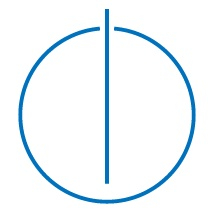
\includegraphics[width=0.2\linewidth]{figures/infologo.jpg}
	\end{figure}
	\bigskip 
\end{center}

\vfill

\newpage
\hoffset=5mm
\thispagestyle{empty}

\begin{center}
	\bigskip \bigskip \bigskip 
	\oTUM{6.0cm} \\
	\vspace*{0.8cm}
	{\huge \bf Technische Universität} \\
	\bigskip
	{\huge \bf München} \\
	\bigskip \bigskip \bigskip
	{\huge \bf Fakultät für Informatik} \\
	\bigskip \bigskip \bigskip
	{\Large \bf Master's Thesis in Informatik} \\
	\bigskip \bigskip \bigskip \bigskip \bigskip
	{\Large An Email-Centered Approach to Intelligent Task Management Using Crowdsourcing and Natural Language Processing} \\
	\bigskip \bigskip \bigskip
	{\Large Ein Email-basierter Ansatz für intelligente Aufgabenverwaltung mit Hilfe von Crowdsourcing und Natural Language Processing} \\
	\bigskip
\end{center}
\vfill

\begin{tabular}{ll}
{\Large \bf Author:} & {\Large John Doe} \\\\
{\Large \bf Supervisor:} & {\Large Prof. Dr. Johann Schlichter} \\\\
{\Large \bf Advisor:} & {\Large Dr. Wolfgang Wörndl} \\\\
{\Large \bf Submission:} & {\Large DD.MM.YYYY}
\end{tabular}

\newpage	
\thispagestyle{empty}
\hoffset=0mm
\vspace*{\fill}
\noindent I assure the single handed composition of this master's thesis only supported by declared resources.\\\\
München, DD.MM.YYYY\\\\\\\\\\\\
\noindent \textit{(John Doe)}

\newpage
\thispagestyle{empty}
\null

\newpage
\thispagestyle{empty}
\hoffset=0mm
\section*{Abstract}	
\begin{spacing}{1.2}
English abstract.
\end{spacing}
	
\section*{Inhaltsangabe}
\begin{spacing}{1.2}
Deutsches Abstract.
\end{spacing}

\newpage
\setcounter{page}{1}
\hoffset=0mm
\bibliographystyle{wmaainf} % quotation style
\setcounter{tocdepth}{3}
\setcounter{secnumdepth}{3}
\fboxsep 0mm


\newpage
\newglossaryentry{SNR}{ name = {SNR}, description={Signal-to-Noise-Ratio}}



\tableofcontents

\newpage
\setlength{\baselineskip}{3ex}

\begin{spacing}{1.15}
	%\input{chapter1}
	%\input{chapter2}
	%\input{chapter3}
	%\input{chapter4}
\end{spacing}
\newpage
\thispagestyle{empty}
\null

\newpage
\addcontentsline{toc}{chapter}{List of figures}
\listoffigures

%\input{appendices}

\newpage
\thispagestyle{empty}
\null
\newpage
\chapter{Introduction}
\section{Motivation}
\section{Contributions}

\newpage
\chapter{Channelmodel}
\begin{figure}[H]
	\centering
	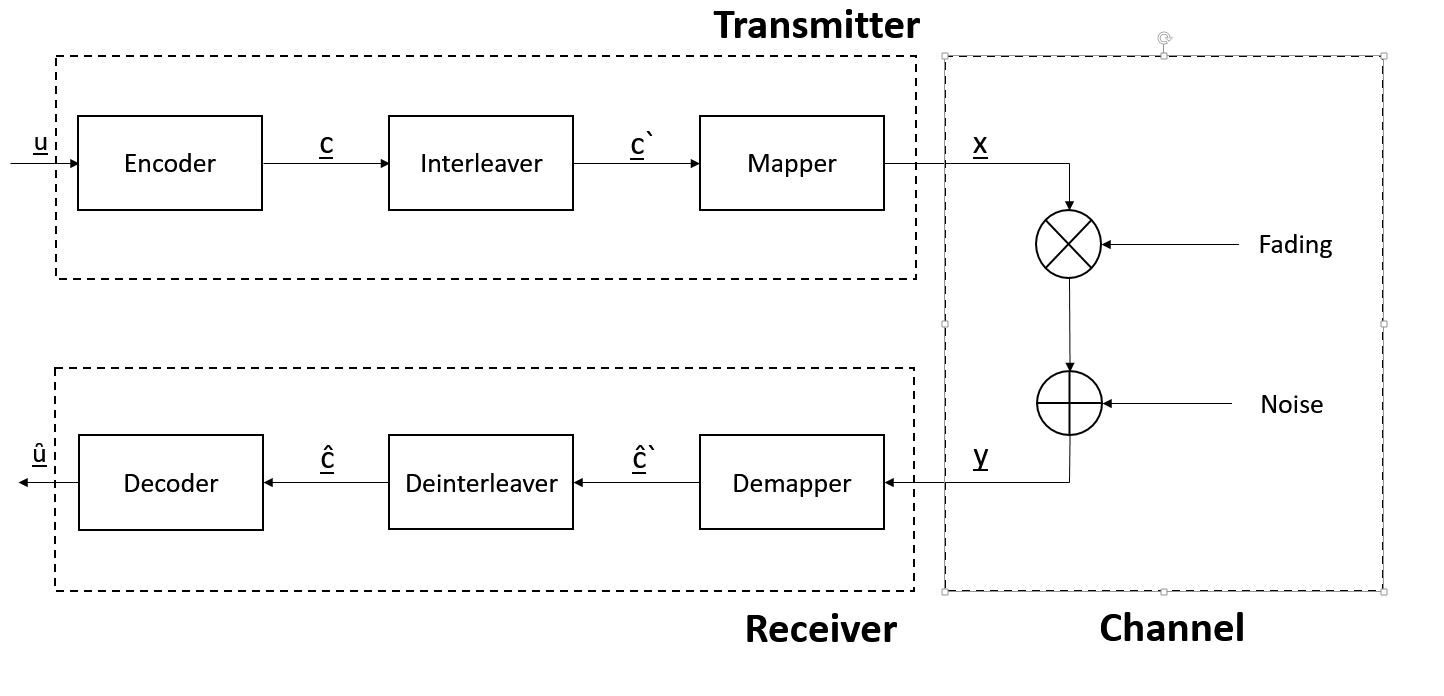
\includegraphics[width=0.7\textwidth]{Channelmodel.PNG}
	\caption{Channelmodel for general Transmitter/Receiver Chain}
	\label{fig:Channelmodel}
\end{figure}

For my purpose we are looking at a simple model which will include a Mapper/Demapper, Encoder/Decode, Interleaving, and the needed channel. We will briefly go over all blocks depicted in the graphic above.

\section{Encoder/Decoder}

For our Encoder/Decoder block we will be looking at a WiMax LDPC code according to the standard IEEE 802.16e. This standard code is used in small and medium distances in urban areas and fits our model quite well. LDPC, which stands for Low Density Parity Check, is a linear error correction code. While it has heavy computing demands, with the growth of computing power it sees more and more use in everyday use. In our case with WiMax we have different given blocksizes ranging from 576 codewords upto 2304. The rates given are 1/2, 2/3, 3/4, and 5/6. We also only look at coding class A for our simulations. 
With a given codeword \textit{x} of length \textit{n} and a generator matrix $G = [I^T|P]$. The parity check matrix texit{H} can now be derived as $H = [-P^T|I\textsubscript{n-k}]$. With the parity check matrix \textit{H} and a code \textit{C} $= xG$ the condition for $cH^t = 0$ must be fulfilled for the codeword to be valid.  
This whole process in MATLAB can be computed with the help of the Coded Modulation Library (CML). For this we have the given function "\textit{InitializeWiMaxLDPC}" to create the parity-check.matrix, "\textit{LdpcEncode}" and "\textit{MpDecode}" to encode and decode our codeword.


\section{Bitinterleave/Deinterleaver}

With the help of bitinterleaving we can avoid any kind of "bursterrors", i.e. we avoid any longer blockerrors. The interleaving in MATLAB is accomplished by creating a random permutation array \textit{k}. The permutation array can be used to randomly shuffle our codeword and also return them back to default at receiver side.

\newpage

\section{Mapper/Demapper}

The mapper or modulation is used to assign a specific codelength a symbol which is transmitted. The symbols are located in a real/imaginary plane. With the distance from the nullpoint of the axis giving the amplitude of our signal and the angle to the real axis the phase shift. 
There are many forms of modulation schemes, with the most common ones being M-PSK, M-FSK, M-AM and M-QAM. For our simulations we will have a further look in QPSK, 16-QAM and 64-QAM, which are depicted below.

\begin{figure}[H]
	\centering
	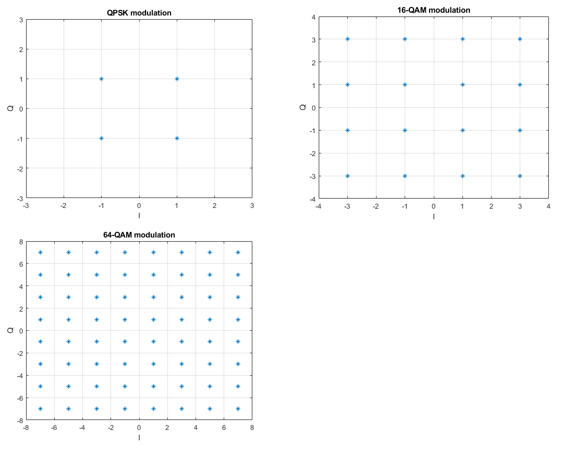
\includegraphics[width=0.95\textwidth]{Modulation_schemes.PNG}
	\caption{Modulation in I/Q planes for QPSK, 16-QAM and 64-QAM}
	\label{fig:Modulation}
\end{figure}

QPSK, which stands for Quadrature Phase shift keying is one of the easier models we will be looking at. The symbols all share the same amplitude and only differ in their respective phase angle. With the information entropy $S = log\textsubscript{2}(M)$ we can identify the maximum number of bits we can assign in every symbol, with M being the number of symbols in the modulation scheme. So for QPSK the number of bits per symbol amounts to 2.

With M-QAM, Quadrature Amplitude Modulation, we add the phase shift already implemented into QPSK the additional differntiation with the amplitude of symbols. For QAM we send signals which differ in their phase shift and also the amplitude.  For 16-QAM we get a maximum of 3 bits per symbols and for 64-QAM 4 bits per symbol.
The modulation schemes makes it possible to increase our rate of transmission and is used for any kind of practical transmission of information.

\section{Channel}
The channel can be modified in many different ways. We can different sources of noise or fading, which can relate to realworld interferences. Some interferences experienced in real life transmission are e.g. thermal noise, distance, doppler effect and reflection of signals. To approach those kind of interferences there are many different channel models in simulations, like an AWGN-Channel or Rayleigh/Rician fading. We will havea further look into the AWGN-Channel and the Rayleigh fading.

\subsection{AWGN-Channel}
The easiest channel manipulition is to add random gaussian noise to the channel, also commonly known as AWGN-Channel (Additive White Gaussian Noise). Like the name says we will add noise which is randomly distributed in a gaussian distribution. The probability density function is defined as follows:
\begin{gather*}
f(x|\mu,\sigma^2) = \frac{1}{\sqrt{2\pi\sigma^2}}*e^{-\frac{(x-\mu)^2}{2\mu}}
\end{gather*}
With x being the aquired point, $\mu$ being the mean or expection of the distribution and $\sigma^2$ the variance of the distribution. For our gaussian noise we will take a mean of 0 and a variance of 1, which will simplify further calculations in the following chapters. We will also always look at complex gaussian noise in our simulations. More or less every communication link will have some kind of gaussian noise interference, so we will add the AWGN-Channel to every simulation we run.

\subsection{Rayleigh-Channel}
Another common channel model used in communication theory is Rayleigh fading. Rayleigh fading is used to simulate multipath reception, which means that for a receiver antenna in a wireless link there are many reflected and scattered signals reaching it. This results into construction or destruction of waves. Rayleigh distribution can be defined like this: $R = \sqrt{X^2 + Y^2}$ with X and Y being two independent gaussian distributed random variables. Further calculations will lead to the following pdf:
\begin{gather*}
f(x;\sigma) = \frac{1}{\sigma^2}e^{-\frac{x^2}{2\sigma^2}} 
\end{gather*} 

	
\newpage
\chapter{Capacity in an AWGN channel}

We will now look into the maximum capacity we can achieve for our communication model in Chapter 2 with added AWGN noise.

\section{Capacity and Monte-Carlo-Simulation}

In general capacity \textit{C} can be defined as the rate \textit{R} at which information can be reliably transmitted over a channel, which means as long $R \leq \ $C we can achieve a transmission without errors even with noise. All the capacities we wil be looking at will be for complex channel models.

For a AWGN-Channel we will have a simple channel model defined by Y = X + N with X $\sim$ \textit{N}(0,$\sigma\textsubscript{T}^2$) and N $\sim$ \textit{N}(0,1). With this our received signal Y will have a distribution of Y $\sim$ \textit{N}(0,$\sigma\textsubscript{T}^2$+1) under the condition that X and N being independently distributed.
We will calculate the capacity as the maximum of mutual information I between X and Y:
\begin{equation}
\label{metric}
C = max(I(X;Y))     
\end{equation}
with X and Y being to independent randomly normal distributed variables.
With the maximum mutual information we calculate the maximum information we can achieve with the given parameters, like modulation, encoding, channel. 
\newline
For the mutual information we can further part it into the differential entropy:
\begin{equation}
\label{metric}
I(X;Y) = h(Y) - h(Y|X)
\end{equation}
\newline
\begin{equation}
\label{metric}
h(Y) = h(X+N) = log(\pi*e^{\sigma^2+1}) \quad \textrm{and} \quad h(Y|X) = h(N) = log(\pi*e^{1})
\end{equation}
Further calculations will lead us to the final equation for the capacity in an AWGN-channel:
\begin{equation}
\label{metric}
C = log(1+\frac{\sigma^2}{N})
\end{equation}
With this approach we have good approximation values for further calculations with added modulation schemes. It is given that for only AWGN the capacity is at his maximum, there should be no capacity value over the calculated ones here. 

\subsection{Approach in Matlab}
The above mentioned formula 2.4 will be simply implemented in MATLAB. With our noise being randomly distributed around 1 our formula simplifies even more into:
\begin{equation}
\label{metric}
C\textsubscript{AWGN} = log(1+SNR) 
\end{equation} 
The SNR here must be transformed into power and not in decibel.

\section{Capacity for QPSK and M-QAM}
Now we will look into different modulation schemes, which were already mentioned in Chapter 1.3. We will implement these modulation schemes into our capacity calculations in an AWGN channel.
\subsection{QPSK}
For QPSK we will have 4 symbols and resulting 2 codebits per symbol. Before any simulation or calculation were run we can already be sure that we will not pass the upper bound of 2 bits/Symbol. So the plot will approach the 2 bits/Symbol for high SNR.
After creating a random codeword modulated with the fitting modulation scheme. Noise is added to the signal, which is than received as the bit array Y. The next step to calculate the capacity differs from above. 
\newline
We know that our signal is normal random distributed variables and we have to calculate the differential entropy for h(Y), which is:
\begin{equation}
\label{metric}
h(Y) =  \sum_{n=0}^N(-log(p(y\textsubscript{n}))) * \frac{1}{N}
\end{equation} 
with p(y) being the probability of y for a normal distributed variable and N the codelength.
\begin{equation}
\label{metric}
p(y) = \frac{1}{n*\pi}*\sum_{i=1}^n(e^{y-x\textsubscript{i}})
\end{equation} 
Here we need to watch out for the number of symbols in the modulation scheme. For QPSK we have a n = 4, 16-QAM n = 16 and 64-QAM n = 64.
\newline
For the QAM modulation only the above mentioned n must be changed.
 

\subsection{Results}
\begin{figure}[H]
	\centering
	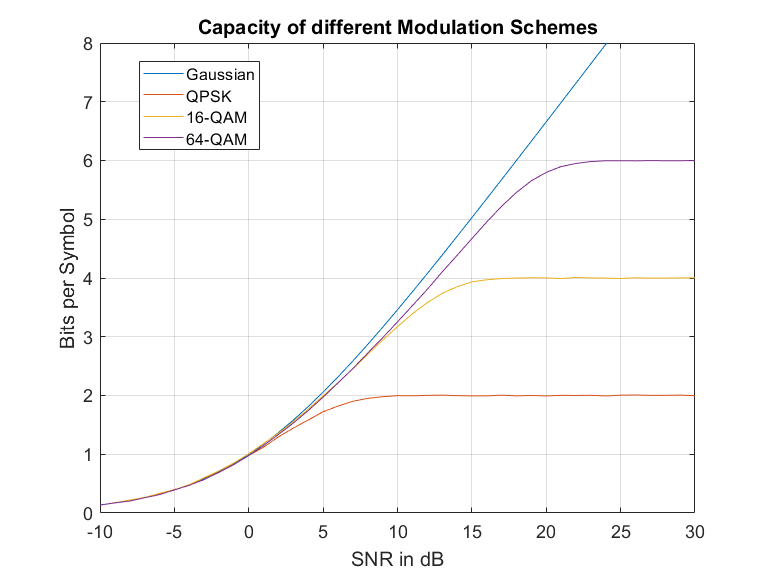
\includegraphics[width=0.7\textwidth]{Capacity_QPSK_QAM.png}
	\caption{Capacity plot for general AWGN-channel, QPSK, 16-QAM and 64-QAM}
	\label{fig:Modulation}
\end{figure}
The results of the calculation in MATLAB can be seen above. We can clearly see the modulated channel approaches the desired bit/symbol rate in a good speed. The gaussian channel clearly outperforms the modulated channels, clearly seen after 0 dB SNR.



\chapter{Transmitter Receiver Chain in MATLAB}

We will now focus in creating a functioning Transmitter-Receiver chain to simulate a wireless communication as real as possible. The blocks for the communication link were shortly introduced in the beginning, but will be explained further in the following chapters.


\section{LDPC and the CML Library}
For our communication protocol we will be using WiMax LDPC. 



\section{FER and comparison with capacity plots}
\begin{figure}[H]
	\centering
	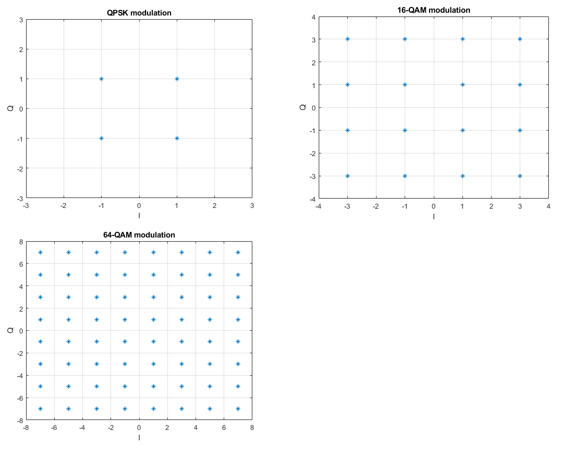
\includegraphics[width=0.95\textwidth]{Modulation_schemes.PNG}
	\caption{Modulation in I/Q planes for QPSK, 16-QAM and 64-QAM}
	\label{fig:Modulation}
\end{figure}

\chapter{Communication link for Rayleigh fading channels}

\section{Rayleigh fading and implementation}

\subsection{Channel estimation}

\section{Rayleigh fading FER with AWGN channel}

\section{Problems and challenges}

\section{Results and comparison with AWGN channel}


\chapter{Conclusion}

\section{Comparison between fading and AWGN channel}

\section{Fazit}




 
















% Generierung des Literaturverzeichnisses
%\bibliography{/path/to/your/.bib/file}

\end{document}
